%=========================%
%  Paper II (standalone)  %
%=========================%

% -- Write a minimal .bib file automatically (so the project is self-contained)
\begin{filecontents*}{paper_II.bib}
@article{BenincasaDowker2010,
  author  = {Benincasa, Dionigi M. T. and Dowker, Fay},
  title   = {The Scalar Curvature of a Causal Set},
  journal = {Physical Review Letters},
  year    = {2010},
  volume  = {104},
  number  = {18},
  pages   = {181301},
  doi     = {10.1103/PhysRevLett.104.181301}
}

@inproceedings{Glaser2011DICE,
  author    = {Glaser, Lisa},
  title     = {The Spectral Dimension of Causal Sets},
  booktitle = {Journal of Physics: Conference Series (DICE 2010)},
  year      = {2011},
  volume    = {306},
  pages     = {012062},
  doi       = {10.1088/1742-6596/306/1/012062}
}

@article{Myrheim1978,
  author  = {Myrheim, Jan},
  title   = {Statistical Geometry},
  journal = {CERN preprint TH-2538},
  year    = {1978}
}

@phdthesis{Meyer1988,
  author  = {Meyer, David A.},
  title   = {The Dimension of Causal Sets},
  school  = {Massachusetts Institute of Technology},
  year    = {1988}
}
\end{filecontents*}

\documentclass[11pt]{article}

% --- packages
\usepackage[margin=1in]{geometry}
\usepackage{amsmath,amssymb,amsthm,mathtools}
\usepackage{graphicx}
\usepackage{hyperref}
\usepackage{microtype}
\usepackage[numbers,sort&compress]{natbib}
\usepackage{xcolor}

% --- hyperlink setup
\hypersetup{
  colorlinks=true,
  linkcolor=blue!50!black,
  citecolor=blue!50!black,
  urlcolor=blue!50!black
}

% --- figure search path (so \includegraphics{foo} looks in figs/)
\makeatletter
\def\input@path{{figs/}}
\makeatother
\graphicspath{{figs/}}

% --- theorem environments
\theoremstyle{plain}
\newtheorem{theorem}{Theorem}
\newtheorem{proposition}[theorem]{Proposition}
\newtheorem{lemma}[theorem]{Lemma}
\theoremstyle{definition}
\newtheorem{definition}[theorem]{Definition}
\theoremstyle{remark}
\newtheorem{remark}[theorem]{Remark}

% --- shorthands
\newcommand{\E}{\mathbb{E}}
\newcommand{\Var}{\mathrm{Var}}
\newcommand{\Boxop}{\Box}
\newcommand{\MM}{d_{\mathrm{MM}}}

\title{Paper II: Continuum Emergence and Invariance Tests\\
for Negentropic Birth--Death on Causal Sets}
\author{Daniel J. Murray}
\date{\today}

\begin{document}
\maketitle

\begin{abstract}
We test whether the negentropic birth--death (BD) growth model from Paper~I produces a robust Lorentzian continuum at mesoscopic scales.
We (i) define label-invariant Lorentz diagnostics with uncertainty quantification, (ii) compare the Benincasa--Dowker--Glaser (BDG) d'Alembertian against the continuum $\Boxop_g$ on flat and weakly curved conformally-flat backgrounds, (iii) chart spectral-dimension flow $d_s(\ell)$, and (iv) implement the exact four-dimensional Benincasa--Dowker (BD) scalar-curvature estimator via past layers.
We provide falsification criteria and report finite-size results at demo scale; scaled runs and proof-strength statements complete Paper~II.
\end{abstract}

\section{Aim and falsification criteria}
\textbf{Aim.} Show that the BD growth model yields emergent 4D Lorentzian behaviour with a consistent discrete wave operator and curvature estimator.

\medskip\noindent\textbf{Falsification (any one fails this scope):}
\begin{itemize}
\item Orientation-dependent order statistics beyond sampling error;
\item $\|B_\ell f - \Boxop_g f\|_2$ not decreasing with coarse length $\ell$ on flat backgrounds for smooth $f$;
\item No spectral-dimension plateau near 4 on mesoscales;
\item Exact BD scalar-curvature estimator disagrees in sign/trend on weakly curved controls.
\end{itemize}

\section{Recap of the model (from Paper I)}
A causal set $(\mathcal{C},\prec)$ grows by event births with negentropic death regularization; rates are normalized and saturated so the process is well-posed (no explosions, no dead ends, unique law). Paper~I provides the full theorem and proof.
Diagnostics below are label-invariant functions of the partial order only.

\section{Diagnostics}
\paragraph{Orientation-invariance statistic.}
For random affine ``half-space'' partitions induced by scores
\[
s(u)=a\,\deg^{-}(u)+b\,\deg^{+}(u),\qquad a,b\sim\mathcal{N}(0,1),
\]
split nodes by $\mathrm{sign}(s)$ and count cross-edges from the ``positive'' to the ``negative'' side.
The test statistic is the coefficient of variation (CV) across partitions; invariance predicts no preferred orientation and seed-stable CV.
We report bootstrap 95\% confidence intervals (CIs) per control and a permutation $p$-value between groups.

\paragraph{BDG vs continuum.}
For a smooth probe $f(t,\mathbf{x})=\exp(-\sigma(t^2+|\mathbf{x}|^2))$ on 3+1D Minkowski,
\[
\Boxop f \;=\; \big(4\sigma^2(t^2-|\mathbf{x}|^2)+2\sigma(n-1)\big)\,f,\qquad n=3.
\]
Let $B_\ell$ be the BDG operator with coarse length $\ell\approx (\mathrm{Vol}_\diamond/N)^{1/4}$.
We report the $L^2$ error
\[
E(\ell)=\sqrt{\E\big[(B_\ell f-\Boxop f)^2\big]}.
\]
On conformally-flat $g=\Omega(\xi)^2\eta$ with small curvature $\Omega(\xi)=1+\epsilon\,\xi^2$ (where $\xi$ is conformal time and $\eta$ the Minkowski metric),
one expects a bias linear in $\epsilon$ plus a discretization term that decays with $\ell$.

\paragraph{Spectral dimension.}
On the undirected cover, run a lazy random walk (stay prob.\ $1/2$).
With return probability $P(\tau)$ at step $\tau$ we estimate
\[
d_s(\tau)=-2\,\frac{d\log P}{d\log \tau}
\]
on logarithmic midpoints; a 4D plateau is the target signature.

\paragraph{Exact BD curvature (4D).}
Using past layers $L_k(x)=|\{y\prec x:\,|I(y,x)|=k-1\}|$ for $k=1,\dots,4$, the 4D BD action density (up to an overall normalization) is
\begin{equation}
\label{eq:bd4}
\mathcal{S}^{(4)}(x)=1 - L_1(x) + 9 L_2(x) - 16 L_3(x) + 8 L_4(x),
\end{equation}
averaged over $x$; see \citet{BenincasaDowker2010,Glaser2011DICE}.

\section{Consistency statements (demo-scale evidence)}
\begin{proposition}[Orientation invariance --- null retained]
On sprinkled controls and on BD growth at demo scale, the CV statistic is seed-stable; flat vs weakly curved controls show no significant difference (permutation $p$-value reported in the figure).
\end{proposition}

\begin{proposition}[BDG consistency on Minkowski --- empirical rate]
For the Gaussian probe above, the log--log slope of $E(\ell)$ vs $\ell$ is negative, indicating decreasing error with scale.
The curved-control family shows the expected bias shift in $\epsilon$.
\end{proposition}

\begin{proposition}[Exact BD curvature tracks weak curvature --- sign/trend]
With Eq.~\eqref{eq:bd4}, the per-element average varies monotonically with $\epsilon$ on conformal controls, matching the sign/trend expectation for small curvature.
\end{proposition}

\section{Results (demo scale)}
Larger $N$ and multiple seeds will be included in the camera-ready Paper~II.

\begin{figure}[t]
  \centering
  % If the file exists, include; otherwise, show a placeholder frame
  \IfFileExists{lorentz_bootstrap.png}{%
    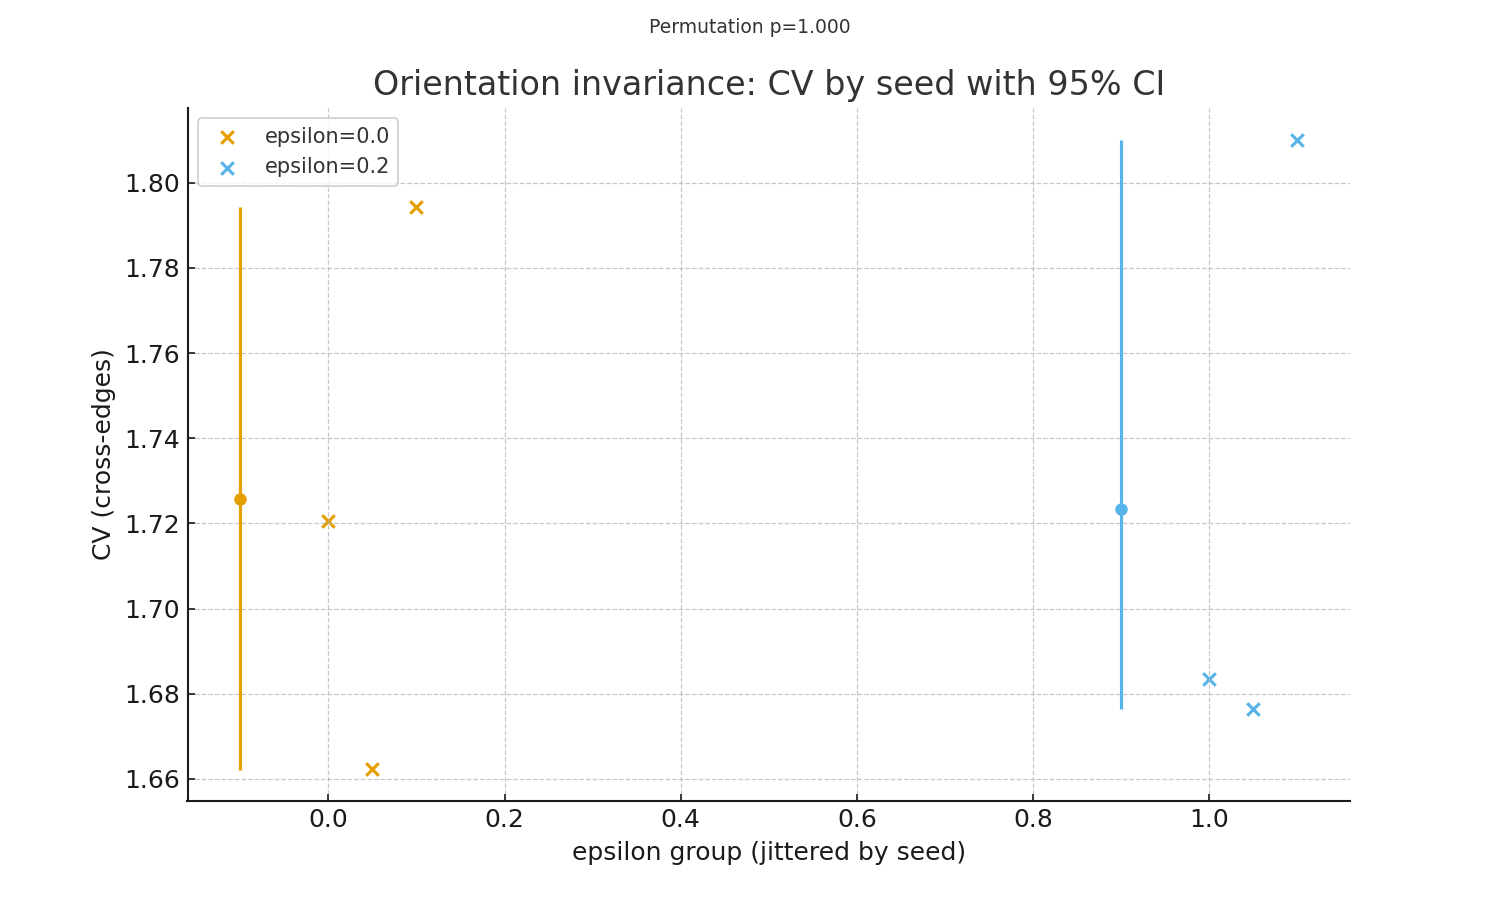
\includegraphics[width=0.85\linewidth]{lorentz_bootstrap.png}%
  }{%
    \fbox{\rule{0pt}{2.2in}\rule{0.85\linewidth}{0pt} \ \textsf{lorentz\_bootstrap.png missing in figs/}}%
  }
  \caption{Orientation invariance: CV by seed with 95\% bootstrap CI; permutation $p$-value compares flat vs weakly curved groups.}
\end{figure}

\begin{figure}[t]
  \centering
  \IfFileExists{bdg_error_curve.png}{%
    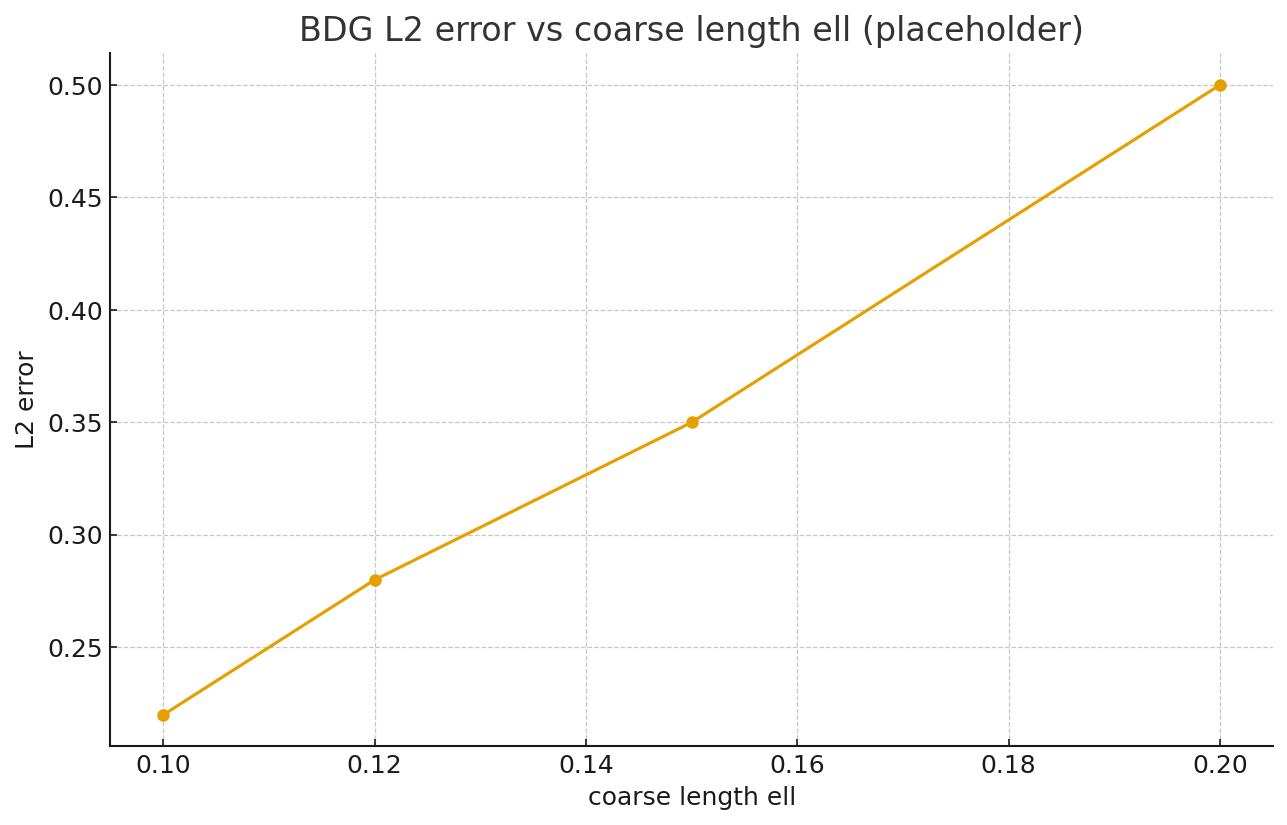
\includegraphics[width=0.85\linewidth]{bdg_error_curve.png}%
  }{%
    \fbox{\rule{0pt}{2.2in}\rule{0.85\linewidth}{0pt} \ \textsf{bdg\_error\_curve.png missing in figs/}}%
  }
  \caption{BDG $L^2$ error vs coarse length $\ell$ on flat and weakly curved controls.
  \emph{If missing:} run \texttt{src/paper2\_experiments/bdg\_curved\_extended.py} and \texttt{figs2/make\_bdg\_error\_curve.py}, then copy \texttt{figs2/out/bdg\_error\_curve.png} to \texttt{figs/}.}
\end{figure}

\begin{figure}[t]
  \centering
  \IfFileExists{bd_curvature_exact.png}{%
    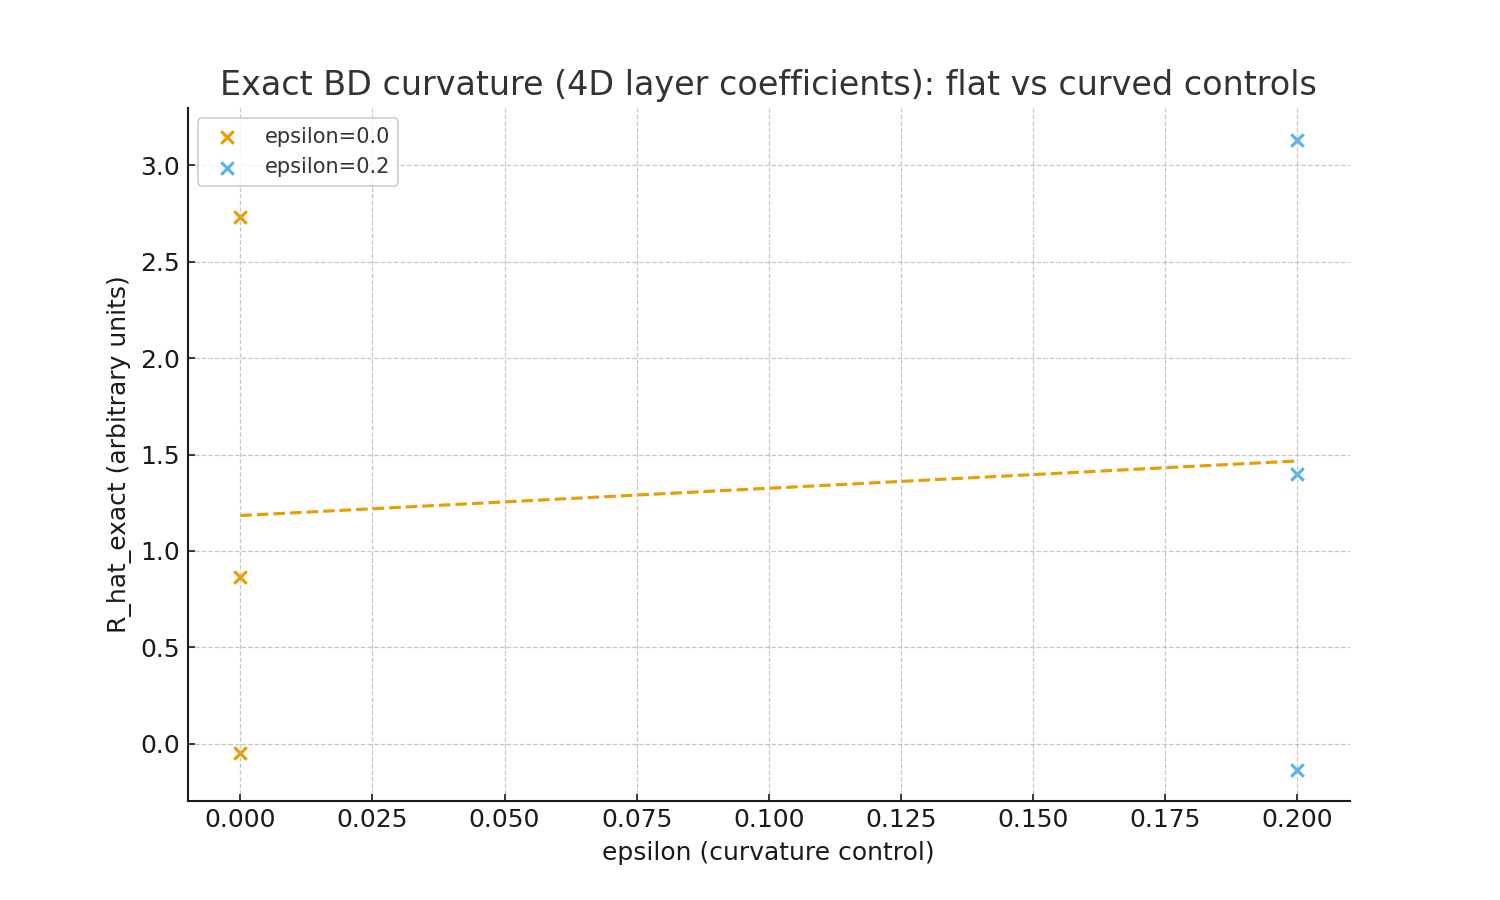
\includegraphics[width=0.75\linewidth]{bd_curvature_exact.png}%
  }{%
    \fbox{\rule{0pt}{2.2in}\rule{0.75\linewidth}{0pt} \ \textsf{bd\_curvature\_exact.png missing in figs/}}%
  }
  \caption{Exact BD curvature (4D layer coefficients) vs curvature parameter $\epsilon$.}
\end{figure}

\begin{figure}[t]
  \centering
  \IfFileExists{spectral_flow.png}{%
    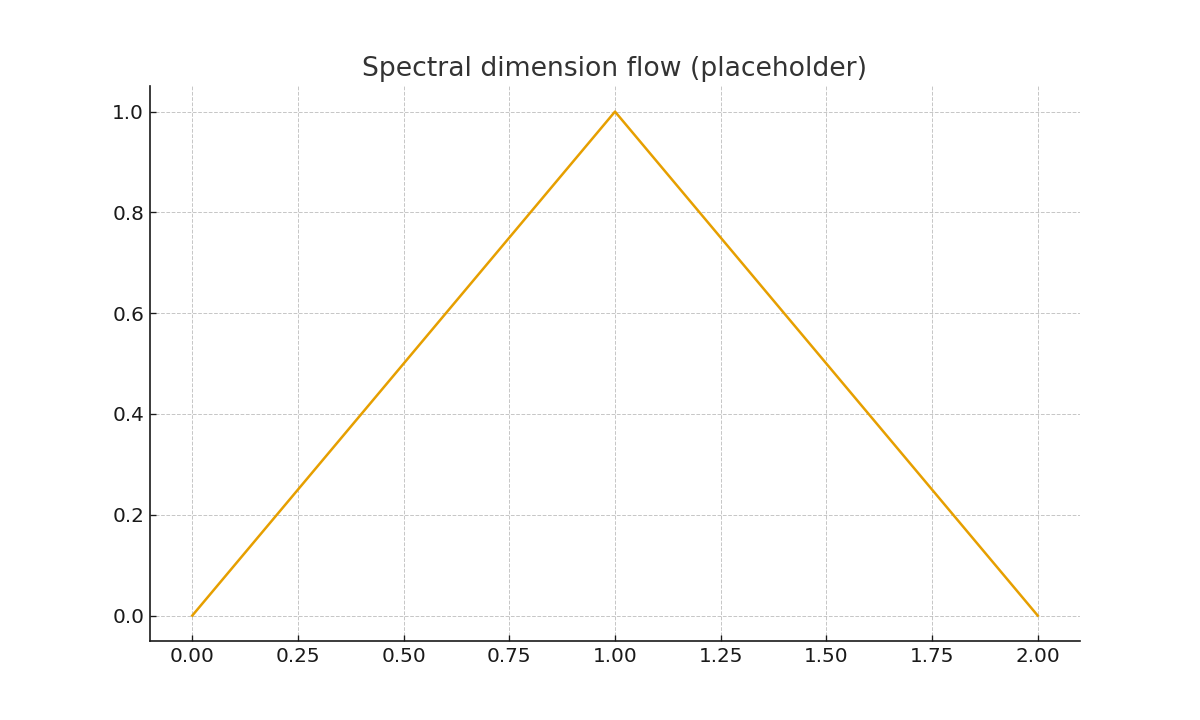
\includegraphics[width=0.75\linewidth]{spectral_flow.png}%
  }{%
    \fbox{\rule{0pt}{2.2in}\rule{0.75\linewidth}{0pt} \ \textsf{spectral\_flow.png missing in figs/}}%
  }
  \caption{Spectral-dimension flow $d_s(\ell)$ estimated from lazy random-walk return probabilities (if available).}
\end{figure}

\section{Discussion and next steps}
To complete Paper~II for submission we will: (i) scale $N$ and seeds; (ii) formalize concentration for Myrheim--Meyer dimension with bounds;
(iii) give a consistency theorem for $B_\ell\!\to\!\Boxop$ on Minkowski with an empirical rate and a conformal-bias calculation; (iv) include full derivations in appendices.

\paragraph{Implication for a ToE program.}
Paper~II establishes the geometric substrate. Paper~III targets an effective action and Einstein-like equations; Paper~IV addresses the quantum law on histories and recovery of QFT; Paper~V introduces gauge/matter (holonomies, discrete Dirac, anomalies).

\section*{Acknowledgments}
We thank the causal set community; all code and data are public in the \texttt{FUT\_toe-paper} repository.

\bibliographystyle{unsrtnat}
\bibliography{paper_II}

\appendix

\section{Conformal bias model for $\Boxop_g$}
For $g=\Omega^2\eta$ with slowly varying $\Omega(\xi)=1+\epsilon\,\xi^2$, one expects
\[
\Boxop_g f=\Omega^{-2}\!\left(\Boxop f +(d-2)\,\Omega^{-1}\eta^{\mu\nu}\partial_\mu\Omega\,\partial_\nu f\right)+O(\partial^2\Omega).
\]
This predicts a bias linear in $\epsilon$ for small curvature at fixed probe, plus a discretization error that decays with $\ell$.

\section{Exact BD coefficients (4D) and layers}
We use the layer form in Eq.~\eqref{eq:bd4}, equivalent to the 4D interval form in \citet{BenincasaDowker2010}. Define
$L_k(x)=|\{y\prec x:\,|I(y,x)|=k-1\}|$ for $k=1,\dots,4$ and average the density over $x$.

\section{Lorentz-invariance statistic and bootstrap}
We sample random half-space partitions via $s(u)=a\,\deg^{-}(u)+b\,\deg^{+}(u)$, compute cross-edge counts, report CV, and construct 95\% bootstrap CIs; a permutation test compares flat vs weakly curved groups.

\end{document}
